%%%%%%%%%%%%%%%%%%%%%%%%%%%%%%%%%%%%%%%%%%%%%%%%%%%%%%%%%%%%%%%%%%%%%%%%
% RÉSULTATS ET DISCUSSIONS
%%%%%%%%%%%%%%%%%%%%%%%%%%%%%%%%%%%%%%%%%%%%%%%%%%%%%%%%%%%%%%%%%%%%%%%%

% ======================================================================
\section{Résultats}
% ======================================================================

Un des objectifs de notre projet consistait à comparer les performances du point de vue temps de calcul et temps de communication des différents algorithmes. Nous nous sommes concentrés sur la comparaison des temps de calcul.
On s'est principalement intéressé la version à une seule étape.

\subsection{Résultats théoriques}

Selon les travaux de nos tuteurs, nous devions obtenir

\begin{figure}[H]
  \begin{center}
    \begin{tabular}{|c|c|c|} \hline
      Algorithme & temps de calcul (ordre de grandeur) One Step  \\
      \hline
      Standard & $2n^{2} + (C_{x} + C_{+})n^{3}$ \\
	  \hline
	  SP & $ (1+C_{\epsilon})n^2 + (C_{x} + C_{exp})n^{3} $ \\
	  \hline  
    \end{tabular}
  \end{center} 
\end{figure}

\noindent n: la valeur maximum entre le nombre de lignes de M, le nombre de colonnes de M et le nombre de colonnes de N dans le cas $P=MN$ \\
$C_{+}$ : complexité temporelle d'une addition \par
\noindent $C_{x}$ : complexité temporelle d'une multiplication \par
\noindent $C_{\epsilon}$ : complexité temporelle du chiffrement \par
\noindent $C_{exp}$ : complexité temporelle d'une exponentiation \par
\noindent $C_{\Delta}$ : complexité temporelle  du déchiffrement

\bigskip
Sachant que d'après \cite{complex-operations} et \cite{FAHIMA}, les complexités sont de l'ordre de :
\begin{itemize}
\item $C_{+} = O(n)$ pour l'addition deux nombres à n chiffres;
\item $C_{x} = O(n²)$ pour la multiplication  deux nombres à n chiffres;
\item $C_{exp} = O(log(n))$ avec n l'exposant. 
\end{itemize}

\subsection{Résultats réels}

Pour confirmer ou invalider les résultats théoriques expliqués dans la publication ~\cite{publi-tuteurs}, nous devons calculer le temps d'exécution d'un job MapReduce en fonction du nombre de lignes des matrices.
Nous avons alors créé une fonction qui permet de stocker les matrices sous la forme adéquate (cf. figure~\ref{ codage M et N } ) 
Afin de nous assurer de la qualité de nos mesures, nous avons mené une étude statistique. 
Cela implique une automatisation du lancement des jobs MapReduce via le programme mis en annexe~\ref{clusterlauncher}.
<<<<<<< HEAD
Nous avons ainsi pu mener notre étude statistique en créant les programmes qui figurent en annexe~\ref{stat1} et en annexe~\ref{Stat.sh}, qui permettent de calculer la moyenne, la variance et l'écart type sur 150 échantillons contenant chacun dix mesures.
Les résultats obtenus (annexe~\ref{txtmesuresMoy} ) nous ont permis de tracer les courbes se trouvant en annexe~\ref{txtmesures}.
Les faibles variances (annexe~\ref{txtmesuresVar}) trouvées montrent que les mesures sont concentrées autour de la moyenne. 
=======
Nous avons ainsi pu mener notre étude statistique en créant les programmes qui figurent en annexe~\ref{stat1} et en annexe~\ref{Stat.sh} qui permettent de calculer la moyenne, la variance et l'écart type sur 150 échantillons contenant chacune dix mesures.
Les resultats obtenus (annexe~\ref{txtmesuresMoy} ), nous ont permis de tracer les courbes qui se trouvent en annexe~\ref{txtmesures}.
Les faibles variances (annexe~\ref{txtmesuresVar}) trouvées montrent les mesures sont concentrées autour de la moyenne. 
>>>>>>> RdgBranche
 
\subsection{Cryptosystème de Paillier}

Pour réaliser l'objectif précédent, nous avons dû, avant tout, implémenter un cryptosystème de Paillier \cite{code-Paillier}, de telle sorte qu'il assure les propriétés homomorphiques.
Pour cela, nous nous sommes aidés d'un code \cite{code-Paillier} que nous avons modifié.

\begin{figure}[H]
\centering
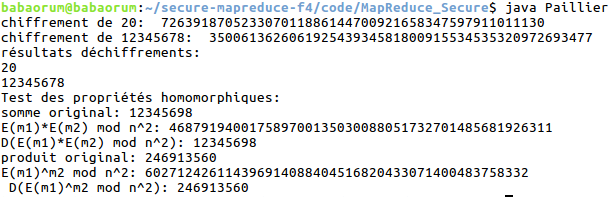
\includegraphics[scale=0.4]{img/res-paillier.png}
\caption{cryptosytème de Paillier et ses propriétés homomorphiques}
\label{Paillier}
\end{figure}



% ----------------------------------------------------------------------
	\subsection{Délivrables}
% ----------------------------------------------------------------------

Au cours de notre projet, de nombreuses réalisations nous ont été demandées pour que nos tuteurs puissent facilement utiliser MapReduce et comparer les résultats de leurs recherches. 
En plus de la mise en place du cluster, nous avons dû créer un programme qui permet d'installer et configurer hadoop : \textit{hadoopFromScratch.sh} (cf. \ref{hfs1}).
Il a fallu également réaliser des scripts qui permettent de lancer les jobs MapReduce en local et sur le cluster: \textit{launcher.sh} (cf. \ref{launcher1}), \textit{clusterLauncher.sh} (cf. \ref{clusterlauncher}).

 
